\twocolumn[\colorsection{Primer principio de la termodinámica}]
\setcounter{figure}{0}
%
\begin{Exercise}
  Un tanque de $\SI{20.0}{\liter}$ contiene $\SI{4.86E-4}{\kilogram}$ de helio a $\SI{18.0}{\celsius}$. La masa molar del helio es $\SI{4.00}{\gram/\mole}$. \textit{a}) ¿Cuántos moles de helio hay en el tanque? \textit{b}) ¿Cuál es la presión en el tanque en pascales y en atmósferas?
\end{Exercise}
\begin{Answer}
	\begin{minipage}[t]{.4\textwidth}
    \textit{a}) $\SI{0.122}{\mole}$\\ \textit{b}) $\SI{14750}{\pascal}$ o $\SI{0.146}{atm}$
  \end{minipage}
\end{Answer}
%
\begin{Exercise}
  \ifthenelse{\equal{\seleccionados}{true}}
  {\addToList{xyz-primerppio}{\ExerciseHeaderNB}}{}
  Un tanque cilíndrico tiene un pistón ajustado que permite modificar el volumen del tanque. Originalmente, el tanque contiene $\SI{0.110}{\cubic\metre}$ de aire a $\SI{0.355}{atm}$ de presión. Se tira lentamente del pistón hasta aumentar el volumen del aire a $\SI{0.390}{\cubic\metre}$. Si la temperatura permanece constante, ¿qué valor final tiene la presión?
\end{Exercise}
\begin{Answer}
  $\SI{0.100}{atm}$
\end{Answer}
%
\begin{Exercise}
  Un matraz de $\SI{1.50}{\liter}$, provisto de una llave de paso, contiene etano gaseoso ($\text{C}_2\text{H}_6$) a $\SI{300}{\kelvin}$ y presión atmosférica ($\SI{101.3}{\kilo\pascal}$). La masa molar del etano es $\SI{30.1}{\gram/\mole}$. El sistema se calienta a $\SI{490}{\kelvin}$, con la llave abierta a la atmósfera. Luego se cierra la llave y el matraz se enfría a su temperatura  original. \textit{a}) Calcule la presión final del etano en el matraz. \textit{b}) ¿Cuántos gramos de etano quedan en el matraz?
\end{Exercise}
\begin{Answer}
	\begin{minipage}[t]{.4\textwidth}
    \textit{a}) $\SI{62}{\kilo\pascal}$\\ \textit{b}) $\SI{1.12}{\gram}$
  \end{minipage}
\end{Answer}
%
\begin{Exercise}
  Dos moles de gas ideal se calientan a presión constante desde $\SI{27.0}{\celsius}$ hasta $\SI{107}{\celsius}$. Calcule el trabajo efectuado por el gas.
\end{Exercise}
\begin{Answer}
  $\SI{1330}{\joule}$
\end{Answer}
%
\begin{Exercise}
  \ifthenelse{\equal{\seleccionados}{true}}
  {\addToList{xyz-primerppio}{\ExerciseHeaderNB}}{}
  Seis moles de gas ideal están en un cilindro provisto en un extremo con un pistón móvil. La temperatura inicial del gas es $\SI{27.0}{\celsius}$ y se desplaza el pistón manteniendo la presión del gas constante. Calcule la temperatura final del gas una vez que haya efectuado $\SI{2.4}{\kilo\joule}$ de trabajo.
\end{Exercise}
\begin{Answer}
  $\SI{75.1}{\celsius}$
\end{Answer}
%
\begin{Exercise}\label{p:primerppio01}
  La gráfica de la figura \ref{f:primerppio01} muestra un diagrama $p$-$V$ del aire en un pulmón cuando una persona inhala y luego exhala una respiración profunda. Estas gráficas, obtenidas en la práctica clínica, normalmente están algo curvadas, pero modelamos una como un conjunto de líneas rectas de la misma forma general. (Importante: La presión indicada es la presión manométrica, no la presión absoluta). \textit{a}) ¿Cuántos joules de trabajo neto realiza el pulmón de esta persona durante una respiración completa? \textit{b}) El proceso que aquí se representa es algo diferente de los que se han estudiado, ya que el cambio de presión se debe a los cambios en la cantidad de gas en el pulmón, y no a los cambios de temperatura. (Piense en su propia respiración, sus pulmones no se expanden porque se han calentado). Si la temperatura del aire en el pulmón permanece en un valor razonable de $\SI{20}{\celsius}$, ¿cuál es el número máximo de moles en el pulmón de esta persona durante una respiración?
\end{Exercise}
\begin{Answer}
	\begin{minipage}[t]{.4\textwidth}
    \textit{a}) $\SI{1}{\joule}$\\ \textit{b}) $\SI{0.06}{\mole}$
  \end{minipage}
\end{Answer}
%
\begin{center}
  \begin{tikzpicture}[scale=0.9]
    \begin{axis}[
                 every major x tick/.append style={thick,blue},
                 clip=false,
                 grid=both,
                 minor x tick num=3,        %un minor tick es decir 0.5
                 minor y tick num=3,
                 xmin=0, xmax=1.6,           %min y max para los ejes, NO PARA EL DOMINIO
                 ymin=0, ymax=13, 
                 %axis y line=center,        %alinea el eje al centro de la figura
                 %axis x line=middle,        %sino pone 2 ejes x
                 xtick  align=center,
                 xlabel={$V$~[L]},
                 ylabel={$p$~[mmHg]}         
                ];
    \addplot [color=blue, thick] [id=pulmon1,samples= 180, domain=0.1:0.4]  {1+80/3*(x-0.1)};
    \addplot [color=blue, thick] [id=pulmon2,samples= 180, domain=0.4:1.4]  {9+2*(x-0.4)};
    \addplot [color=blue, thick] [id=pulmon3,samples= 180, domain=1:1.4]  {2+90/4*(x-1)};
    \addplot [color=blue, thick] [id=pulmon4,samples= 180, domain=0.1:1]  {1+10/9*(x-0.1)};
    \draw [red, -{Stealth}] (0.15,4)--(0.25,20/3) node[midway,sloped,above] {inhalación};
    \draw [red, -{Stealth}] (0.6,10)--(0.85,10.5) node[midway,sloped,above] {inhalación};
    \draw [red, -{Stealth}] (1.15,7.25)--(1.05,5) node[midway,sloped,above] {exhalación};
    \draw [red, -{Stealth}] (0.7,2.33)--(0.4,2) node[midway,sloped,above] {exhalación};
    \end{axis}
  \end{tikzpicture}
  \captionof{figure}{Problema \ref{p:primerppio01}\label{f:primerppio01}}
\end{center}
%
\begin{Exercise}
  Durante el tiempo en que $\SI{0.305}{\mole}$ de un gas ideal experimentan una compresión isotérmica a  $\SI{22}{\celsius}$, su entorno efectúa $\SI{468}{\joule}$ de trabajo sobre él. \textit{a}) Si la presión final es $\SI{1.76}{atm}$, ¿cuál fue la presión inicial? \textit{b}) Realice una gráfica $p$-$V$ para este proceso.
\end{Exercise}
\begin{Answer}
	\begin{minipage}[t]{.4\textwidth}
    \textit{a}) $\SI{0.941}{atm}$
  \end{minipage}
\end{Answer}
%
\begin{Exercise}
  Cuando se hierve agua a una presión de $\SI{2.00}{atm}$, el calor de vaporización es $\SI{2.20}{\mega\joule/\kilogram}$ y la temperatura del punto de ebullición es $\SI{120}{\celsius}$. A esta presión, $\SI{1.00}{\kilogram}$ de agua ocupa un volumen de $\SI{1.00E-3}{\cubic\metre}$, y $\SI{1.00}{\kilogram}$ de vapor de agua ocupa un volumen de $\SI{0.824}{\cubic\metre}$. Calcule el incremento en la energía interna del agua cuando se forma $\SI{1.00}{\kilogram}$ de vapor de agua a esta temperatura.
\end{Exercise}
\begin{Answer}
	\begin{minipage}[t]{.4\textwidth}
    $\Delta U = \SI{2.03E6}{\joule}$ (es menor al calor recibido)
  \end{minipage}
\end{Answer}
%
\begin{Exercise}\label{p:primerppio02}
  \ifthenelse{\equal{\seleccionados}{true}}
  {\addToList{xyz-primerppio}{\ExerciseHeaderNB}}{}
  Considere el ciclo cerrado $a\rightarrow b \rightarrow c \rightarrow d \rightarrow a$ mostrado en la figura \ref{f:primerppio02}. \textit{a}) Encuentre una expresión para el trabajo total efectuado por el sistema en este proceso. \textit{b}) Encuentre una expresión para el trabajo total efectuado por el sistema si el  ciclo se recorre en sentido opuesto.
\end{Exercise}
\begin{Answer}
	\begin{minipage}[t]{.4\textwidth}
    \textit{a}) $W_{abcda} = (p_1-p_0)(V_1-V_0)$\\ \textit{b}) $W_{adcba} = -W_{abcda}$
  \end{minipage}
\end{Answer}
%
\begin{center}
  \begin{tikzpicture}[scale=0.9]
    \begin{axis}[
      axis x line=bottom,
      axis y line=left,
      xmin=0, xmax=6,           %min y max para los ejes, NO PARA EL DOMINIO
      ymin=0, ymax=9, 
      xlabel={$V$},
      ylabel={$p$},
      xtick={1,5},
      xticklabels={$V_0$,$V_1$},
      ytick={2,7},
      yticklabels={$p_0$,$p_1$}
      ]
    % \draw [color=blue, very thick][-latex](160pt,20pt)..controls(100pt,25pt) and (60pt,45pt)..(42pt,58pt);
    \draw [color=blue, very thick][-latex](5,2)--(3,2);
    \draw [color=blue, very thick](3,2)--(1,2);
    \draw [color=blue, very thick][-latex] (1,2)--(1,4.5);
    \draw [color=blue, very thick] (1,4.5)--(1,7);
    \draw [color=blue, very thick][-latex] (1,7)--(3,7);
    \draw [color=blue, very thick] (3,7)--(5,7);
    \draw [color=blue, very thick][-latex] (5,7)--(5,4.5);
    \draw [color=blue, very thick] (5,4.5)--(5,2);
    \draw [dashed, thick] (1,0)--(1,2);
    \draw [dashed, thick] (5,0)--(5,2);
    \draw [dashed, thick] (0,2)--(1,2);
    \draw [dashed, thick] (0,7)--(1,7);
    \filldraw(1,2)circle(2pt) (1,7)circle (2pt)(5,7)circle(2pt)(5,2)circle(2pt);
    \draw (1,2) node [below left] {$a$};
    \draw (1,7) node [above left] {$b$};
    \draw (5,7) node [above right] {$c$};
    \draw (5,2) node [below right] {$d$};
    \end{axis}
  \end{tikzpicture}
  \captionof{figure}{Problema \ref{p:primerppio02}\label{f:primerppio02}}
\end{center}
%
\begin{Exercise}\label{p:primerppio03}
  En la figura \ref{f:primerppio03} se muestra el diagrama $p$-$V$ del proceso $a\rightarrow b \rightarrow c$ que implica $\SI{0.0175}{\mole}$ de un gas ideal. \textit{a}) ¿Cuál fue la temperatura más baja que alcanzó el gas en  este proceso? ¿Dónde ocurrió? \textit{b}) ¿Cuánto trabajo realizó o recibió el gas en el proceso $a \rightarrow b$? \textit{c}) ¿Cuánto trabajo realizó o recibió el gas en el proceso $b \rightarrow c$? \textit{d}) Si se entregaron $\SI{215}{\joule}$ de calor al gas durante $a\rightarrow b \rightarrow c$, ¿cuántos de esos Joules se destinaron a la energía interna?
\end{Exercise}
\begin{Answer}
	\begin{minipage}[t]{.4\textwidth}
    \textit{a}) $\SI{278}{\kelvin}$ en el estado $a$\\ \textit{b}) $\SI{0}{\joule}$\\ \textit{c}) realizó $\SI{162}{\joule}$ de trabajo\\ \textit{d}) $\SI{53}{\joule}$
  \end{minipage}
\end{Answer}
%
\begin{center}
  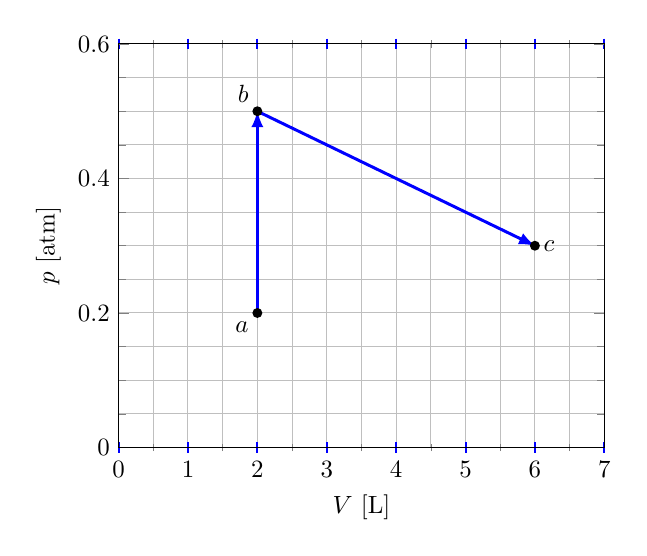
\begin{tikzpicture}[scale=0.9]
    \begin{axis}[
      every major x tick/.append style={thick,blue},
      clip=false,
      grid=both,
      minor x tick num=1,
      minor y tick num=3,
      xmin=0, xmax=7,
      ymin=0, ymax=0.6,
      xtick  align=center,
      xlabel={$V$~[L]},
      ylabel={$p$~[atm]}
      ];
      \draw [color=blue, very thick][-latex](2,0.2)--(2,0.5);
      \draw [color=blue, very thick][-latex](2,0.5)--(6,0.3);
      \draw (2,0.2) node [below left] {$a$};
      \draw (2,0.5) node [above left] {$b$};
      \draw (6,0.3) node [right] {$c$};
      \fill [black](2,0.2) circle(2pt);
      \fill [black](2,0.5) circle(2pt);
      \fill [black](6,0.3) circle(2pt);
    \end{axis}
  \end{tikzpicture}
  \captionof{figure}{Problema \ref{p:primerppio03}\label{f:primerppio03}}
\end{center}
%
\begin{Exercise}\label{p:primerppio04}
  \ifthenelse{\equal{\seleccionados}{true}}
  {\addToList{xyz-primerppio}{\ExerciseHeaderNB}}{}
  El gráfico en la figura \ref{f:primerppio04} muestra un diagrama $p$-$V$ de $\SI{3.25}{\mole}$ de helio ideal gaseoso. La parte $c \rightarrow a$ de este proceso es isotérmica. \textit{a}) Calcule el calor intercambiado por el helio en los procesos $a \rightarrow b$, $b \rightarrow c$ y $c \rightarrow a$. \textit{b}) Calcule la variación de energía interna del He en esos mismos procesos.
\end{Exercise}
\begin{Answer}
	\begin{minipage}[t]{.4\textwidth}
    \textit{a}) $Q_{ab}=\SI{60.0}{\kilo\joule}$, $Q_{bc}=\SI{-36.0}{\kilo\joule}$ y $Q_{ca}=\SI{-11.1}{\kilo\joule}$\\ \textit{b}) $\Delta U_{ab}=\SI{36.0}{\kilo\joule}$, $\Delta U_{bc}=\SI{-36.0}{\kilo\joule}$ y $\Delta U_{ca}=\SI{0}{\kilo\joule}$
  \end{minipage}
\end{Answer}
%
\begin{center}
  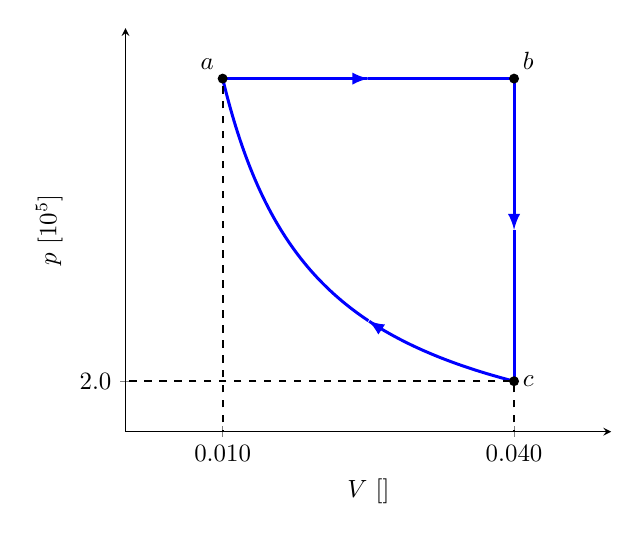
\begin{tikzpicture}[scale=0.9]
    \begin{axis}[
      %ticks=none,
      axis x line=bottom,
      axis y line=left,
      xmin=0, xmax=5,           %min y max para los ejes, NO PARA EL DOMINIO
      ymin=1, ymax=9, 
      xlabel={$V$~[$\si{\cubic\metre}$]},
      ylabel={$p$~[$10^5 \si{\pascal}$]},
      xtick={1,4},
      xticklabels={0.010,0.040},
      ytick={2},
      yticklabels={2.0}
      %yticklabels={},
      %extra x ticks={0.04},
      %extra y ticks={2}
      ];
    \addplot [-latex, color=blue, very thick] [samples= 180, domain=1:2.5]  {8};
    \addplot [color=blue, very thick] [samples= 180, domain=2.5:4]  {8};
    \addplot [color=blue, very thick] [samples= 180, domain=1:2.5]  {8/x};
    \addplot [latex-, color=blue, very thick] [samples= 180, domain=2.5:4]  {8/x};
    \addplot[color = black, dashed, thick] coordinates {(4, 0) (4, 2) (0, 2)};
    \addplot[color = black, dashed, thick] coordinates {(1, 0) (1, 8)};
    \draw [color=blue, very thick][-latex](4,8)--(4,5);
    \draw [color=blue, very thick](4,5)--(4,2);
    \draw (1,8) node [above left] {$a$};
    \draw (4,8) node [above right] {$b$};
    \draw (4,2) node [right] {$c$};
    \fill [black](1,8) circle(2pt);
    \fill [black](4,8) circle(2pt);
    \fill [black](4,2) circle(2pt);
    \end{axis}
  \end{tikzpicture}
  \captionof{figure}{Problema \ref{p:primerppio04}\label{f:primerppio04}}
\end{center}
%
\begin{Exercise}\label{p:primerppio05}
  \textit{a}) Una tercera parte de un mol de gas He evoluciona a lo largo de la trayectoria $a \rightarrow b \rightarrow c$ representada por la línea continua en la figura \ref{f:primerppio05}. Suponga que el gas se puede tratar como ideal. ¿Cuánto calor intercambia gas? \textit{b}) Si, en vez de ello, el gas pasa  del estado $a$ al estado $c$ evolucionando a lo largo de la línea horizontal punteada en la figura, ¿cuánto calor intercambia el gas en este caso?
\end{Exercise}
\begin{Answer}
	\begin{minipage}[t]{.4\textwidth}
    \textit{a}) $\SI{3200}{\joule}$\\ \textit{b}) $\SI{2000}{\joule}$
  \end{minipage}
\end{Answer}
%
\begin{center}
  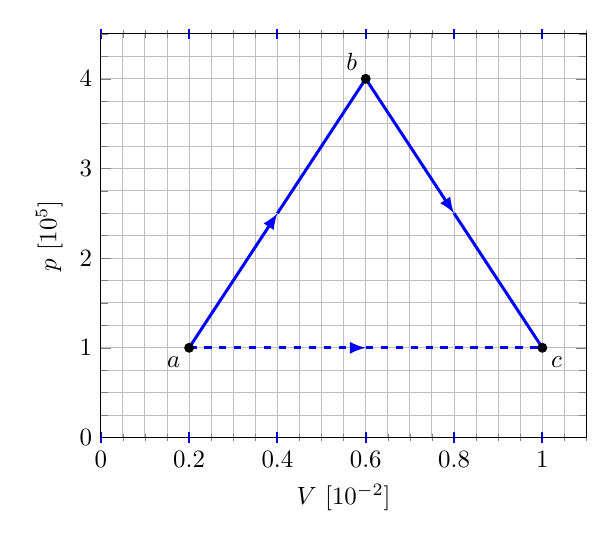
\begin{tikzpicture}[scale=0.9]
    \begin{axis}[
      every major x tick/.append style={thick,blue},
      clip=false,
      grid=both,
      minor x tick num=3,
      minor y tick num=3,
      xmin=0, xmax=1.1,
      ymin=0, ymax=4.5,
      xtick  align=center,
      xlabel={$V$~[$10^{-2} \si{\cubic\metre}$]},
      ylabel={$p$~[$10^5 \si{\pascal}$]}
      ];
      \draw [color=blue, very thick][-latex](0.2,1)--(0.4,2.5);
      \draw [color=blue, very thick](0.4,2.5)--(0.6,4);
      \draw [color=blue, very thick][-latex](0.6,4)--(0.8,2.5);
      \draw [color=blue, very thick](0.8,2.5)--(1,1);
      \draw [color=blue, dashed, very thick][-latex](0.2,1)--(0.6,1);
      \draw [color=blue, dashed, very thick](0.6,1)--(1,1);
      \draw (0.2,1) node [below left] {$a$};
      \draw (0.6,4) node [above left] {$b$};
      \draw (1,1) node [below right] {$c$};
      \fill [black](0.2,1) circle(2pt);
      \fill [black](0.6,4) circle(2pt);
      \fill [black](1,1) circle(2pt);
    \end{axis}
  \end{tikzpicture}
  \captionof{figure}{Problema \ref{p:primerppio05}\label{f:primerppio05}}
\end{center}
%
\begin{Exercise}
  \ifthenelse{\equal{\seleccionados}{true}}
  {\addToList{xyz-primerppio}{\ExerciseHeaderNB}}{}
  Se colocan $\SI{0.20}{\mole}$ de un gas ideal diatómico en un recipiente a $\SI{3.0}{atm}$ y $\SI{500}{\kelvin}$. Se efectúa con el gas el siguiente ciclo: \textit{i}) Se expande isotérmicamente desde el estado \textit{A} hasta duplicar su volumen llegando al estado \textit{B}. \textit{ii}) A volumen constante se reduce su temperatura hasta $\SI{300}{\kelvin}$, alcanzando el estado \textit{C}. \textit{iii}) A presión constante se reduce su volumen hasta el volumen inicial (estado \textit{D}). \textit{iv}) El gas aumenta su temperatura a volumen constante hasta el estado \textit{A}. Para este ciclo se pide: \textit{a}) Realizar un diagrama $p-V$ indicando en qué procesos el gas realiza o recibe trabajo y en cuáles absorbe o cede calor. \textit{b}) Calcular el trabajo neto realizado por el gas. \textit{c}) Calcular el cociente entre el trabajo realizado neto y el calor absorbido por el gas.
\end{Exercise}
\begin{Answer}
	\begin{minipage}[t]{.4\textwidth}
    \textit{b}) $W = \SI{327}{\joule}$\\ \textit{c}) $0.16$
  \end{minipage}
\end{Answer}
%
\begin{Exercise}
  Un mol de un gas ideal diatómico se comprime lentamente a un tercio de su volumen original. En esta compresión, la magnitud del trabajo realizado sobre el gas es $\SI{600}{\joule}$. \textit{a}) Si el proceso es isotérmico, ¿cuál es el valor del calor $Q$ para el gas? ¿El flujo de calor es hacia adentro o hacia afuera del gas? \textit{b}) Si el proceso es isobárico, ¿cuál es el cambio en la energía interna del gas? ¿Aumenta o disminuye su energía interna?
\end{Exercise}
\begin{Answer}
	\begin{minipage}[t]{.4\textwidth}
    \textit{a}) $Q = \SI{-600}{\joule}$, el gas cede calor\\ \textit{b}) $\Delta U = \SI{-1500}{\joule}$, disminuye
  \end{minipage}
\end{Answer}
%
\begin{Exercise}
  Un cilindro con pistón contiene $\SI{0.15}{\mole}$ de nitrógeno a $\SI{0.18}{\mega\pascal}$ y $\SI{300}{\kelvin}$, que se puede tratar como un gas ideal. Primero, el gas se comprime isobáricamente a la mitad de su volumen original. Luego se expande adiabáticamente hasta su volumen original. Por último, se calienta isocóricamente hasta su presión original. Calcule el trabajo del gas en este ciclo.
\end{Exercise}
\begin{Answer}
	\begin{minipage}[t]{.4\textwidth}
    $W = \SI{-74.4}{\joule}$
  \end{minipage}
\end{Answer}
%
